\begin{singlespace}
\chapter*{Background and Context for ``\textit{Causal single-cell RNA-seq simulation, in silico perturbation, and GRN inference benchmarking using GRouNdGAN-Toolkit}''}
\markboth{Background and Context for \textsc{GRouNdGAN-Toolkit}}{Background and Context for \textsc{GRouNdGAN-Toolkit}}
\end{singlespace}

While \textsc{rapppid} represented a meaningful advance in our ability to make accurate predictions on datasets which controlled for data leakage, generalization remained (and continues to remain) a challenge for \textsc{ppi} inference models. Following the publication of \textsc{rapppid}, we began to look to specific areas in which \textsc{ppi} inference models fail to generalize. Predicting interactions between proteins of different organism, particularly those of very evolutionary distance species, had been previously identified as a challenge for \textsc{ppi} inference models \cite{dick_pipe4_2020, sledzieski_d-script_2021}. What's more, these ``cross-species'' interactions are of great value to researchers. The vast majority of \textsc{ppi}s studied belong to a small number of model organisms representing a small fraction of all species, representing less than a third of taxa at the class rank as measured by the \textsc{string} core dataset \cite{intrepppid}. We've named this discrepancy in elucidated \textsc{ppi}'s the ``species gap''. It follows, then, that it would be greatly advantageous to construct computational methods for expanding our knowledge of \textsc{ppi}s in species other than a select few model organisms.

The cross-species \textsc{ppi} inference models of which I was aware at the time, however, conducted their evaluations on datasets which suffered from data leakage \cite{dick_pipe4_2020, sledzieski_d-script_2021}. Further, when evaluated on a strict, \textsc{c3} dataset which controlled for data leakage, performance severely deteriorated \cite{intrepppid}.

This is the context from which our method \textsc{intrepppid} arose \cite{intrepppid}. \textsc{intrepppid} builds upon the lessons and architecture of \textsc{rapppid}, leaving unchanged its \textsc{awd-lstm} encoder, expanding the model such that it now also modelled the orthology between proteins. Orthology here can be thought of similarities in protein sequence across species due them sharing a common ancestor \cite{fang_getting_2010}. Modelling orthology proved to have many synergistic effects with the cross-species task, lending itself particularly well to both theoretical and practical concerns. Theoretically, homology is a natural place to begin when comparing the interactions of two species, and forms the basis of many early analyses such as Date and Marcotte's work as well as that of Sharan \textit{et al.} \cite{date_discovery_2003, sharan_conserved_2005}. Practically, the orthology modelling task can be argued to provide a regularizing effect when viewed through the lens of contrastive self-supervised learning \cite{intrepppid, chen_simple_2020, sermanet_time-contrastive_2018}. Due to our novel ``quintuplet'' architecture, whereby an encoders weights are shared across a twin network task as well as as a triplet contrastive network, the number of parameters used in the \textsc{intrepppid} network were ostensibly identical to that of \textsc{rapppid}. 

\textsc{intrepppid} successfully improved on \textsc{rapppid}'s predictive performance on testing pairs between proteins of the same  and differing organisms \cite{intrepppid}. Experiments also demonstrated that the improvements in predictive performance that \textsc{intrepppid} enjoyed were due to having successfully modelled orthology, rather than any spurious or unintended cause resulting from the novel ``quintuplet'' architecture. \textsc{intrepppid}'s efficient architecture and resulting low computational requirements has allowed us to create an online service, \href{https://ppi.bio}{\textsc{ppi}.bio}, for using \textsc{intrepppid} and \textsc{rapppid} to infer \textsc{ppi} interactions. Together, the work presented in the \textsc{intrepppid} manuscript represent a concrete step in the direction of narrowing the species gap.

%\textsc{intrepppid} demonstrates a novel network construction which was designed with a focus on its ability to model the underlying biological data while using regularization techniques and a limited number of parameters to account for the limited amount of high-quality \textsc{ppi} training pairs are available to us. Together with the tools we've created to make \textsc{ppi} inference more accessible with \href{https://ppi.bio}{\textsc{ppi}.bio}, the work presented in the \textsc{intrepppid} manuscript brings us closer to narrowing the species gap.

\begin{tcolorbox}
    The contents of Chapter 4 were first published on the 22\textsuperscript{nd} of August, 2024 as an article of the same title in Volume 25, Issue 5, of Oxford University Press' \textit{Briefings in Bioinformatics} journal and is made available under the \href{https://creativecommons.org/licenses/by-nc/4.0/legalcode.en}{Creative Commons Attribution-NonCommercial License}, © Joseph Szymborski and Amin Emad, 2024. \textsc{doi}: \href{https://doi.org/10.1093/bib/bbae405}{10.1093/bib/bbae405}
\end{tcolorbox}

\begin{singlespace}
\chapter[Causal single-cell RNA-seq simulation, in silico perturbation, and GRN inference benchmarking using GRouNdGAN-Toolkit]{Causal single-cell RNA-seq simulation, in silico perturbation, and GRN inference benchmarking using GRouNdGAN-Toolkit}
\markboth{Chapter 4: GRouNdGAN-Toolkit}{Chapter 4: GRouNdGAN-Toolkit}%
\end{singlespace}

\counterwithout{section}{chapter}
\renewcommand{\thetable}{\arabic{table}}
\renewcommand{\thefigure}{\arabic{figure}}

\figuresection{Causal single-cell RNA-seq simulation, in silico perturbation, and GRN inference benchmarking using GRouNdGAN-Toolkit}

\section*{Abstract}
\addcontentsline{toc}{section}{Abstract}
An overwhelming majority of protein–protein interaction (\textsc{ppi}) studies are conducted in a select few model organisms largely due to constraints in time and cost of the associated ‘wet lab’ experiments. In silico \textsc{ppi} inference methods are ideal tools to overcome these limitations, but often struggle with cross-species predictions. We present \textsc{intrepppid}, a method that incorporates orthology data using a new ‘quintuplet’ neural network, which is constructed with five parallel encoders with shared parameters. \textsc{intrepppid} incorporates both a \textsc{ppi} classification task and an orthologous locality task. The latter learns embeddings of orthologues that have small Euclidean distances between them and large distances between embeddings of all other proteins. \textsc{intrepppid} outperforms all other leading \textsc{ppi} inference methods tested on both the intraspecies and cross-species tasks using strict evaluation datasets. We show that \textsc{intrepppid}’s orthologous locality loss increases performance because of the biological relevance of the orthologue data and not due to some other specious aspect of the architecture. Finally, we introduce \textsc{ppi}.bio and \textsc{ppi} Origami, a web server interface for \textsc{intrepppid} and a software tool for creating strict evaluation datasets, respectively. Together, these two initiatives aim to make both the use and development of \textsc{ppi} inference tools more accessible to the community.
\newpage
\section*{Graphical Abstract}

\begin{figure}[h]%figure2
	\centerline{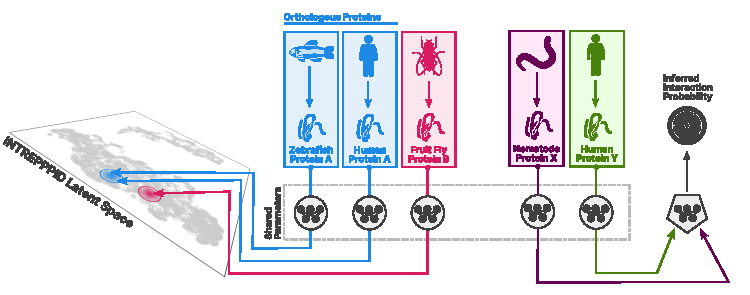
\includegraphics[scale=1]{figures/intrepppid/graphical_abstract.pdf}}
\end{figure}

\textbf{Keywords}: protein-protein interactions; orthology; cross-species; deep learning

\section*{Introduction}
\addcontentsline{toc}{section}{Introduction}
Studying how proteins work in concert has yielded deeply valuable biological insights. Not least of these insights is the implication of protein interactions in the appearance of biological phenotypes and relatedly, how disrupting these interactions can lead to disease [1, 2]. Knowledge of these interactions can, in turn, be used to design drugs and therapies to treat the diseases for which they are implicated [3, 4].

As the relevant technologies have improved, studies which experimentally verify protein–protein interactions (\textsc{ppi}s) have increased in size. In fact, multiple recent studies have published so-called `all-by-all' studies whereby the interaction of entire proteomes are experimentally evaluated. In September 2014, researchers assembled a reference network of ∼14~000 interactions from a search space of 13~000 human genes through a combination of yeast-two-hybrid (\textsc{y2h}) assays and other validation experiments [5]. Five years later, the same network (‘\textsc{h}u\textsc{ri}’) expanded to ∼53~000 interactions from a search space of 17~500 proteins [6].

While these studies provide an invaluable wealth of data, they represent a tremendous investment of time, labour, and money. A major consequence of the high cost of `all-by-all' studies is that it is prohibitively expensive to exhaustively perform them for all known species. In fact, it is currently only practical to limit these studies to a small number of well-studied model organisms. This is a problem common to many aspects of the life sciences, which we've taken to calling `the species gap'.

As of February, 2024 there are currently 793~217 taxa spanning 108~340 genera enumerated by the \textsc{ncbi} Taxon Database [7]. Few, if any, experimental studies are capable of accounting for most, let alone all, of these taxa. For this reason, scientists rely on select few `model' organisms that exhibit desirable properties that lend themselves to a field of study or methodology. These selection criteria further bias our already small sampling of all possible living subjects of study. To demonstrate the extent of the species gap, we quantified the number of distinct organisms that are absent from the \textsc{string} Core \textsc{ppi} database [8], by calculating the intersection of taxa in this database and taxa in the \textsc{ncbi} Taxon Database. We found that only 30\% of all taxa at the class rank and 16\% at the order rank were present in the \textsc{string} Core database (Fig. \ref{fig:intrepppid_species_gap}), underscoring the lack \textsc{ppi} information from the vast majority of species.

Recent advances in co-fractioning and cross-linking mass-pectrometry (\textsc{cf-ms} and \textsc{xl-ms}, respectively) methods have greatly increased the throughput of \textsc{ppi} experiments. Both methods have many advantageous properties for \textsc{ppi} prediction, including their speed, not requiring over-expression, and the ability to identify protein complexes [10].

\textit{In silico} models of protein interaction have many favourable characteristics that may help narrow the species gap. Relative to ‘wet lab’ experiments such as \textsc{y2h} or \textsc{cf/xl-ms}, which may take on the order of days or months to complete and analyse, \textit{in silico} methods can take as little as seconds or minutes. Furthermore, most \textit{in silico} \textsc{ppi} prediction methods operate entirely unattended, resulting in much lower labour costs. Finally, inferring \textsc{ppi}s is often computationally inexpensive and can leverage commodity hardware. In summary, \textit{in silico} methods and their low cost lend themselves to the task of exhaustively searching protein interaction spaces.

Many \textit{in silico} methods, however, face challenges that make them unsuitable for less-studied organisms. Namely, many methods, especially those dependent on machine learning, require a training dataset comprised of \textsc{ppi}s. These datasets must be sufficiently large to provide a representative sample of interactions. They must also scale with the number of parameters being learned lest the model overfit. Other methods that do not rely on machine learning have similar requirements.

\begin{figure}[b]
	\centerline{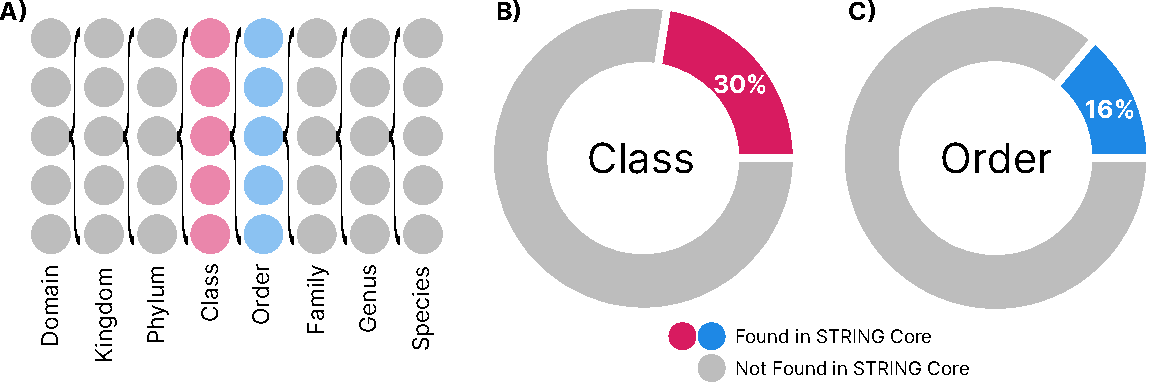
\includegraphics[scale=0.7]{figures/intrepppid/string_species_analysis-eps-converted-to.pdf}
    }
    \caption[The species gap as illustrated by the \textsc{string} \textsc{ppi} database.]{\textbf{\textsf{The species gap as illustrated by the STRING PPI database.}} \textbf{(A)} the hierarchy of biological taxa [9]. \textbf{(B, C)} Doughnut charts indicating the proportion of all taxa represented in \textsc{string} Core at the class rank \textbf{(B)} and order rank \textbf{(C)}.}\label{fig:intrepppid_species_gap}
\end{figure}

Regrettably, a major barrier to bridging the species gap is that there are often too few interaction data to train \textsc{ppi} inference models for lesser-studied organisms. In order for computational models to address the species gap, they must make accurate \textsc{ppi} inferences on less-studied organisms, while using existing \textsc{ppi} data from well-studied organisms during training. Such ‘cross-species’ inference can be used to infer the intraspecies \textsc{ppi} network of the less-studied organism, all while only using the model organism as training data, addressing the species gap. Cross-species inference requires that methods perform accurate out-of-distribution (\textsc{ood}) inference. Historically, \textsc{ppi} inference methods have failed to make accurate predictions on interactions between \textsc{ood} proteins [11–13].

In 2012, a letter published by Park and Marcotte outlined the severity of pervasive data leakage that was obscuring the inability of methods of the time to generalize to interactions between \textsc{ood} proteins [11]. The cause of the data leakage Park and Marcotte observed was the common ‘random splitting’ approach to preparing cross-validation folds. Random splitting of interactions (between pairs of proteins) into folds allows for the same proteins appearing in both the training and testing sets, resulting in data leakage. Park and Marcotte found that when methods of the time were trained and tested on ‘strict’ datasets where proteins present in the training set never appear in any of the other folds, the accuracy of most methods dropped to random levels. This precipitous drop in performance indicates that all the models tested had problems dealing with \textsc{ood} proteins.

While Park and Marcotte found that \textsc{ood} performance was poor across the landscape of methods available in 2012, studies by Dunham and Ganapathiraju in 2021 and Bernett \textit{et al.} in 2023 corroborate the 12-year-old findings [12, 13]. In both studies, contemporary sequence-based \textsc{ppi} inference methods were tested on datasets that satisfy Park and Marcotte’s strictest validation schemes. Predictive power dramatically degraded in all cases, just as Park and Marcotte observed in 2012. While models for \textsc{ppi} inference have changed drastically since 2012 with the notable introduction of deep learning methods, reported performance of methods continue to be inf lated as a result of the random splitting of interactions (as opposed to stricter splitting based on proteins).

Furthermore, work by Hamp and Rost as well as Bernett \textit{et al.} underscore an additional source of data leakage: distinct proteins with sequences which are nearly identical [13, 14]. Amino acid sequences can be overwhelmingly redundant between distinct proteins. An important consequence of this is that two proteins with all but identical sequences may appear in both sets, thereby leaking data in the same way randomly-splitting \textsc{ppi} pairs does. The challenges presented by sequence similarity can be overcome by ensuring that proteins in the training set do not have a sequence identity above some threshold with proteins in the testing set.

One of the earliest approaches for sequence-based \textsc{ppi} inference is Marcotte \textit{et al.}'s `Rosetta Stone' method [15]. The authors outline a theory whereby interacting proteins of one species sometimes appear as fused homologous proteins in other species. Using this technique, Marcotte \textit{et al.} inferred interactions between proteins from \textit{Escherichia coli} using information of proteins of other genomes that had similar sequences to the putative pair. The concept of `interologue' was soon after introduced to describe proteins whose interactions are conserved among their respective orthologues [16]. Interologues allow us to extend knowledge of interactions of one species to other species by identifying both sequences and interactions that are conserved between them [17, 18]. These homology-based methods, while effective at identifying conserved interactions, have limitations related to unknown interactions, as acknowledged in the work that first introduced the term interologue: `Although potentially powerful, applying the interologue concept alone in estimating the significance of potential interactions precludes the finding of novel connections previously unidentified in other model organisms' [16].

Some of the first machine-learning methods for predicting \textsc{ppi}s were kernel-based methods operating on sequence features. The support vector machine (\textsc{svm}) is an algorithm for finding the maximum-margin hyperplane for a classification or regression problem, relying on kernel transformations of the input data to solve nonlinear problems [19]. Effectively applying \textsc{svm}s to the problem of \textsc{ppi} classification depends greatly on the design of the kernels used to represent protein pairs. These kernels, designed by expert knowledge, may compare individual proteins to each other (`genomic kernels') or pairs of proteins to other pairs (`pairwise kernels'). Furthermore, these kernels may compare a variety of features of the gene products being studied, including motifs, gene ontology (\textsc{go}) annotations, sequence similarity, or some combination thereof [20].

As advances in hardware and algorithms made research into deep learning more feasible, they’ve proven to be effective in a number of problem domains, not least of which being \textsc{ppi} prediction. Richoux \textit{et al.} demonstrated that twin neural-networks are far more efficient at \textsc{ppi} inference than other network architectures [21]. Twin neural networks are models that consider pairs of inputs using the same trainable parameters rather than specifying parameters for each input and are commonly used to make comparisons between two inputs [22, 23]. Twin networks can reduce the risk of overfitting and aiding few-shot performance [24]. Many twin \textsc{ppi} prediction methods rely on convolutional neural networks (\textsc{cnn}s) or recurrent neural networks (\textsc{rnn}s) to encode feature sequences. The \textsc{pipr} method by Chen \textit{et al.}, however, eschews these architectures for a hybrid: the recurrent \textsc{cnn} (\textsc{rcnn}) [25]. The \textsc{rcnn} comprises of an initial \textsc{cnn} layer whose output is fed into a bidirectional gated recurrent unit (\textsc{gru}) \textsc{rnn} [26].

We’ve previously described \textsc{rapppid}, a method for \textsc{ppi} prediction that outperforms leading methods on strict validation sets that conform to the guidelines set out by Park and Marcotte [11, 27]. \textsc{rapppid} is a twin network that learns latent representations of sequences and inputs them into a classifier network to infer whether two proteins interact. \textsc{rapppid} achieves its high performance largely due to its adoption of averaged weight-decayed \textsc{lstm} (\textsc{awd-lstm}) and the Unigram tokenization algorithm [28, 29]. The former is a combination of regularization techniques that are effective for long short-term memory (\textsc{lstm}) \textsc{rnn}s. The input is tokenized using subword regularization, which regularizes the network by sampling from a distribution of different segmentations of the input [30].

In spite of the aforementioned progress in the field, most computational models are not designed to address the species gap and exhibit reduced performance when tested on the cross-species task. This makes them unsuitable to address the species gap problem and as such, the knowledge of the protein interactions that govern fundamental biological processes of ill-studied non-model organisms remains beyond our grasp. To address this issue, we introduce an extension of \textsc{rapppid} named \textsc{intrepppid} (Incorporating Triplet Error for Predicting \textsc{ppi}s using Deep Learning). \textsc{intrepppid} is specifically designed to improve cross-species \textsc{ppi} prediction performance with the aim of reducing the species gap. In this study, ‘cross-species’ \textsc{ppi} prediction refers to predicting the intraspecies interactions of proteins of one species using a computational model that is trained on intraspecies interactions of a different species. This term does not refer to predicting the interaction between one protein from one species and another protein from a different species.

We designed \textsc{intrepppid} to learn latent representations of amino acid sequences that are useful for predicting \textsc{ppi}s as well as identifying orthologues. Alongside \textsc{rapppid}’s original twin network for inference, \textsc{intrepppid} adds a triplet network that minimizes the Euclidean distance between latent representations of orthologous sequences while maximizing it for nonorthologous sequences. Parameters are shared between both the twin and triplet networks, resulting in five networks with a single set of shared parameters, which we call a ‘quintuplet’ network. \textsc{intrepppid}’s architecture learns a latent space that encodes both \textsc{ppi} and orthology information. This allows us to enforce an inductive bias loosely based on the concept of interologues.

The contributions of this study are as follows. First, we introduce \textsc{intrepppid}, a deep learning method based on a novel quintuplet architecture and a carefully designed loss function that makes out-of-distribution predictions of \textsc{ppi}s to address the species gap. Our analysis shows that \textsc{intrepppid} outperforms all leading methods tested on both intraspecies and cross-species \textsc{ppi} predictions. Second, we demonstrate that \textsc{intrepppid} effectively learns the orthology of proteins and its performance improvement is due to learning biologically relevant information. This suggests the use of orthology information as a powerful approach for making out-of-distribution predictions in this domain. Third, we have released to the community \textsc{ppi}.bio, an open-source interface for \textsc{intrepppid} and \textsc{rapppid} hosted on the internet. This allows researchers to infer \textsc{ppi}s without installing any specialized software or using the command line. Finally, we have released \textsc{ppi} Origami, a computer programme for creating reproducible strict \textsc{ppi} databases in an automated fashion. By automating the dataset generation process, we hope to reduce common sources of data leakage in datasets used for \textsc{ppi} inference.

\section*{Materials and methods}
\label{sec:intrepppid_methods}
\addcontentsline{toc}{section}{Materials and methods}

\subsection*{The INTREPPPID architecture}
\addcontentsline{toc}{subsection}{The \textsc{intrepppid} architecture}

\textsc{intrepppid} integrates \textsc{rapppid}'s twin network for the \textsc{ppi} Classification task with a triplet neural network used for a novel Orthologous Locality task. Learning the two networks jointly results in five encoder layers with shared parameters in what we’ve come to call a quintuplet network architecture.

\textsc{intrepppid} uses the same \textsc{awd-lstm} encoder as the one used in \textsc{rapppid} to learn vector representations of protein sequences. This encoder is a regularized \textsc{rnn} that has been shown to improve performance on tasks that require inferring interactions between proteins absent from the training set [27]. Before encoding, sequences are first tokenized using the Unigram algorithm as implemented by the SentencePiece library [29, 30]. \textsc{intrepppid} uses the vector representations generated by the encoder for two downstream tasks: the `orthologous locality' task and the `\textsc{ppi} classification' task. The encoder as well as the two tasks are trained in an end-to-end fashion.

\textsc{intrepppid}'s quintuplet architecture means that training the network relies on additional orthology data. At inference time, however, only the protein classification twin network is used, so no information other than the amino acid sequences of the proteins in question are required as input.

\subsection*{The protein–protein interaction classification task}
\addcontentsline{toc}{subsection}{The protein–protein interaction classification task}
\textsc{intrepppid} infers \textsc{ppi}s by learning latent representations of the candidate protein sequences which can be classified by a fully connected neural network outputting the interaction probability. The two amino acid sequences ($s_β$ and $s_γ$ ) are first tokenized into vectors $x_β$ and $x_γ$ using the Unigram algorithm. The Unigram algorithm segments the amino acid of the protein sequence into groups using a vocabulary of 250 tokens. The Unigram algorithm also employs subword regularization. Unigram draws tokens for a given sequence from a probabilistic distribution of all possible combination of tokens in the vocabulary, meaning that the same sequence can be tokenized differently between successive calls to the tokenizer.

Once the tokenized vectors $x_β$ and $x_γ$ are obtained, they are inputted into an encoder ($e(\cdot)$) that outputs a latent vector for each protein ($z_β$ and $z_γ$ , respectively):

\begin{align*}
  z_\beta = e(x_\beta)\\
  z_\gamma = e(x_\gamma).
\end{align*}

Finally, the latent vectors $z_\beta$ and $z_\gamma$ are averaged and inputted into a classifier network $g(\cdot)$ that outputs an interaction probability $\hat{y}$:

$$
y = g\left(\left(z_\beta + z_\gamma \right) /2\right) .
$$

The classifier $g(\cdot)$ is a two-layer, fully connected neural network whose hidden layer is activated by the Mish function [31]. The fully connected neural network outputs a single real number which, once activated by the sigmoid function, represents the probability that the proteins represented by the amino acid sequences $s_\beta$ and $s_\gamma$ interact. This interaction probability as well as the true label are inputted into the binary cross-entropy loss to obtain a loss for the \textsc{ppi} classification network:

$$
\mathcal{l}_\textrm{class} = (\hat{y}, y) = −y \cdot \log(\hat{y}) + (1 − y) \cdot \log (1 − \hat{y}) ,
$$

where $y$ is a binary label representing whether the two proteins truly interact ($y = 1$) or not ($y = 0$).

\subsection*{The orthologous locality task}
\addcontentsline{toc}{subsection}{The orthologous locality task}
\textsc{intrepppid} introduces a novel task to help inform the \textsc{ppi} classification network. The orthologous locality task is to learn a latent space whereby the Euclidean distance between latent representations of proteins that are orthologous to one another are within some margin $m$. Conversely, nonorthologous proteins are to have a Euclidean distance greater than $m$.

To achieve this, we adopt a triplet network and a triplet margin loss $\mathcal{l}_\textrm{ortho}$ following the description of [32]:

$$
\mathcal{l}_\textrm{ortho}(z_a, z_p, z_n ) = \max (d (z_a, z_p) − d (z_a, z_n) + m , 0) ,
$$

where $z_a$ is the latent vector of some `anchor' protein for which there is a known orthologous protein with a latent vector $z_p$, $z_n$ is the latent vector of a randomly chosen protein that is not an orthologue of $z_a$, $m$ is a margin factor and $d$ is the Euclidean distance:

$$
d(u, v) = ||u − v||^2.
$$

For the experiments conducted herein, the margin $m$ was fixed at a value of 1.

The principle of the triplet network is to, at every training step, maximize the distance between two nonorthologous proteins (the `anchor' and `negative' proteins), as well as minimize the distance between two orthologous proteins (the `anchor' and `positive' proteins).

The anchor protein, with amino acid sequence $s_a$, can be any protein in the dataset for which orthology data are known. All orthology data for the experiments conducted herein are from the Orthologous Matrix (\textsc{oma}) database of orthologues [33]. In the event that orthologues are known for the protein that $s_\beta$ encodes, $s_\beta$ is chosen to be $s_a$.

The positive and negative proteins (with amino acid sequences $s_p$ and $s_n$, respectively) are chosen relative to $s_a$. $s_p$ is chosen to be the sequence of a randomly chosen protein that, according to the \textsc{oma} database, belongs to the set of sequences of proteins orthologous to the anchor protein. At every training step, $s_p$ is drawn randomly from this set of proteins orthologous to $s_a$, meaning that the positive protein for a given anchor protein may not be the same between training steps or epochs. The negative protein is sampled in a similar manner to the positive protein, but rather than being sampled from the set of proteins orthologous to $s_a$, is sampled from the set of proteins not orthologous to $s_a$. The amino acid sequence of the anchor, positive, and negative proteins ($s_a$, $s_p$, and $s_n$) are tokenized and encoded in the same manner as $s_\beta$ and $s_\gamma$ , resulting in their latent representations $z_a$, $z_p$, and $z_n$.

Optimizing the triplet margin loss in this manner maximizes the Euclidean distance between latent vectors of proteins that are not orthologues, while minimizing the distance between vectors of orthologues. Our adoption of the triplet margin loss follows evidence that such a loss is an effective way of creating feature descriptors that are `spread out' over the latent space, which in turn increases performance on downstream classification tasks [32, 34]. Furthermore, orthologues typically share the same protein functions and therefore offer a good interspecies basis for the downstream \textsc{ppi} classification task [35, 36].

\subsection*{INTREPPPID’s loss function}
\addcontentsline{toc}{subsection}{\textsc{intrepppid}’s loss function}

The final \textsc{intrepppid} loss function that is optimized at training time is the sum of $\mathcal{l}_\textrm{ortho}$ and $\mathcal{l}_\textrm{class}$,

$$
\hat{L}(\hat{y},y,z_a,z_p,z_n) = \mathcal{l}_\textrm{class}(\hat{y},y) + \mathcal{l}_\textrm{ortho}(z_a, z_p, z_n).
$$

In this way, \textsc{intrepppid} optimizes both the orthologous locality and \textsc{ppi} classification losses simultaneously, in an end-toend fashion, ensuring that latent vectors simultaneously encode orthology and \textsc{ppi} information.

\subsection*{Preparing strict protein–protein interaction datasets}
\addcontentsline{toc}{subsection}{Preparing strict protein–protein interaction datasets}

Experiments were run using datasets with strict data splitting folds, described as `\textsc{c3}' by Park and Marcotte [11]. Namely, we ensured that there was no overlap of proteins between any of the training, validation, or testing datasets. Additionally, we controlled for sequence similarity of proteins between the training, validation, and testing sets that is a known vector for information leakage [13, 14]. We specifically control to ensure that proteins with $>90\%$ sequence identity are not present between splits to ensure that proteins that differ only by name are not accidentally present in two different splits. Another reason for choosing a threshold of 90\% sequence identity is that it allows us to test the ability of \textsc{intrepppid} to learn motifs and domains relevant to interactions. Individuals who wish to create testing datasets that limit the exposure of similar motifs and domains can create those with more strict sequence identity requirement (\textit{e.g.} a 50\% threshold) using \textsc{ppi} Origami (see Generating Strict Protein–Protein Interaction Datasets with Protein–Protein Interaction Origami). Protein interaction data are obtained from the \textsc{string} database, version 12 [8]. Interactions with a confidence score $<90\%$ are filtered. \hyperref[sec:intrepppid_supp_methods]{Supplementary Methods} provide details of how we created such strict datasets, and Supplementary Table \hyperref[sec:intrepppid_supp_s1]{S1} outlines summary statistics for the datasets used in this study.

\subsection*{Generating strict protein–protein interaction datasets with protein–protein interaction origami}
\addcontentsline{toc}{subsection}{Generating strict protein–protein interaction datasets with protein–protein interaction origami}
We have written a command-line interface (\textsc{cli}) tool named `\textsc{ppi} Origami' with the aim of making the task of preparing strict \textsc{ppi} datasets in a replicable and automated fashion. \textsc{ppi} Origami has three primary functions: `downloading' primary databases, `processing' primary databases into strict datasets, and an `analysis' function.

\textsc{ppi} Origami allows for the downloading of primary databases as an integrated part of its pipeline. By directly handling downloading third-party databases, \textsc{ppi} Origami ensures that different users of the software are downloading the same files in the same way. \textsc{ppi} Origami also stores downloaded files in a distinct location from the processed files, isolating primary files from accidental changes.

\textsc{ppi} Origami’s main function is to process and transform primary databases into strict \textsc{ppi} datasets. It can create datasets that satisfy both criteria of strict \textsc{ppi} datasets, filtering low-confidence positive examples, and drawing negative examples as previously described.

\textsc{ppi} Origami allows for simple reporting of basic statistics of \textsc{ppi} datasets it generates. These reports allow for convenient verification of whether datasets meet both criteria of strict datasets, as well as other statistics of interest such as the ratio of interactions between dataset cross-validation subsets.

We hope that \textsc{ppi} Origami encourages other researchers to incorporate strict \textsc{ppi} datasets in the future development and analyses of supervised \textsc{ppi} inference methods.

\subsection*{Training procedure}
\addcontentsline{toc}{subsection}{Training procedure}
\textsc{intrepppid} was trained using the Ranger21 optimizer, which uses AdamW with a look-ahead mechanism [37, 38]. An `explore-and-exploit' learning rate scheduler was used, with a maximum learning rate of 0.01 [39]. \textsc{intrepppid} was trained for 100 epochs. The weights of the epoch with the lowest validation loss were used in the analyses herein (and for evaluation on the test set). Hyperparameters used to train \textsc{intrepppid} were informed by those selected during the development of \textsc{rapppid} and are listed in Supplementary Table \ref{tab:intrepppid_supp_hyperparameters}.

\section*{Results}
\addcontentsline{toc}{section}{Results}

\subsection*{INTREPPPID outperforms leading models for prediction of human protein–protein interaction}
\addcontentsline{toc}{subsection}{\textsc{intrepppid} outperforms leading models for prediction of human protein–protein interaction}

First, we set out to evaluate the performance of \textsc{intrepppid} (Fig. \ref{fig:intrepppid_architecture_intra}A) in an intraspecies \textsc{ppi} prediction task: trained and tested on \textit{Homo sapiens} interactions in the \textsc{string} database (see Materials and Methods). Table \ref{tab:intrepppid_perf} shows the performance of \textsc{intrepppid} against five leading \textsc{ppi} prediction methods. These methods include \textsc{rapppid}, our previous method upon which \textsc{intrepppid} expands, \textsc{d-script}, a method designed for the cross-species task, \textsc{pipr}, a twin network with an \textsc{rcnn} encoder, \textsc{sprint}, a sequence-similarity-based method, and the twin networks proposed by Richoux \textit{et al.} [21, 25, 27, 40, 41]. \textsc{intrepppid} performed slightly better than \textsc{rapppid} across all metrics and outperformed all other methods (Table \ref{tab:intrepppid_perf}, Fig. \ref{fig:intrepppid_architecture_intra}B, Supplementary Table \hyperref[sec:intrepppid_supp_s3]{S3}). Richoux \textit{et al.}, \textsc{d-script}, and \textsc{sprint} perform similarly on average, with \textsc{d-script} exhibiting a particularly high degree of variability across the different datasets tested. We observed severe over-fitting while training and testing \textsc{pipr} on all datasets. Precision–recall and receiver-operator Curves are reported in Supplementary Figs \ref{fig:intreppid_supp_pr} and \ref{fig:intreppid_supp_roc}, respectively.

\begin{figure}[h!]
	\centerline{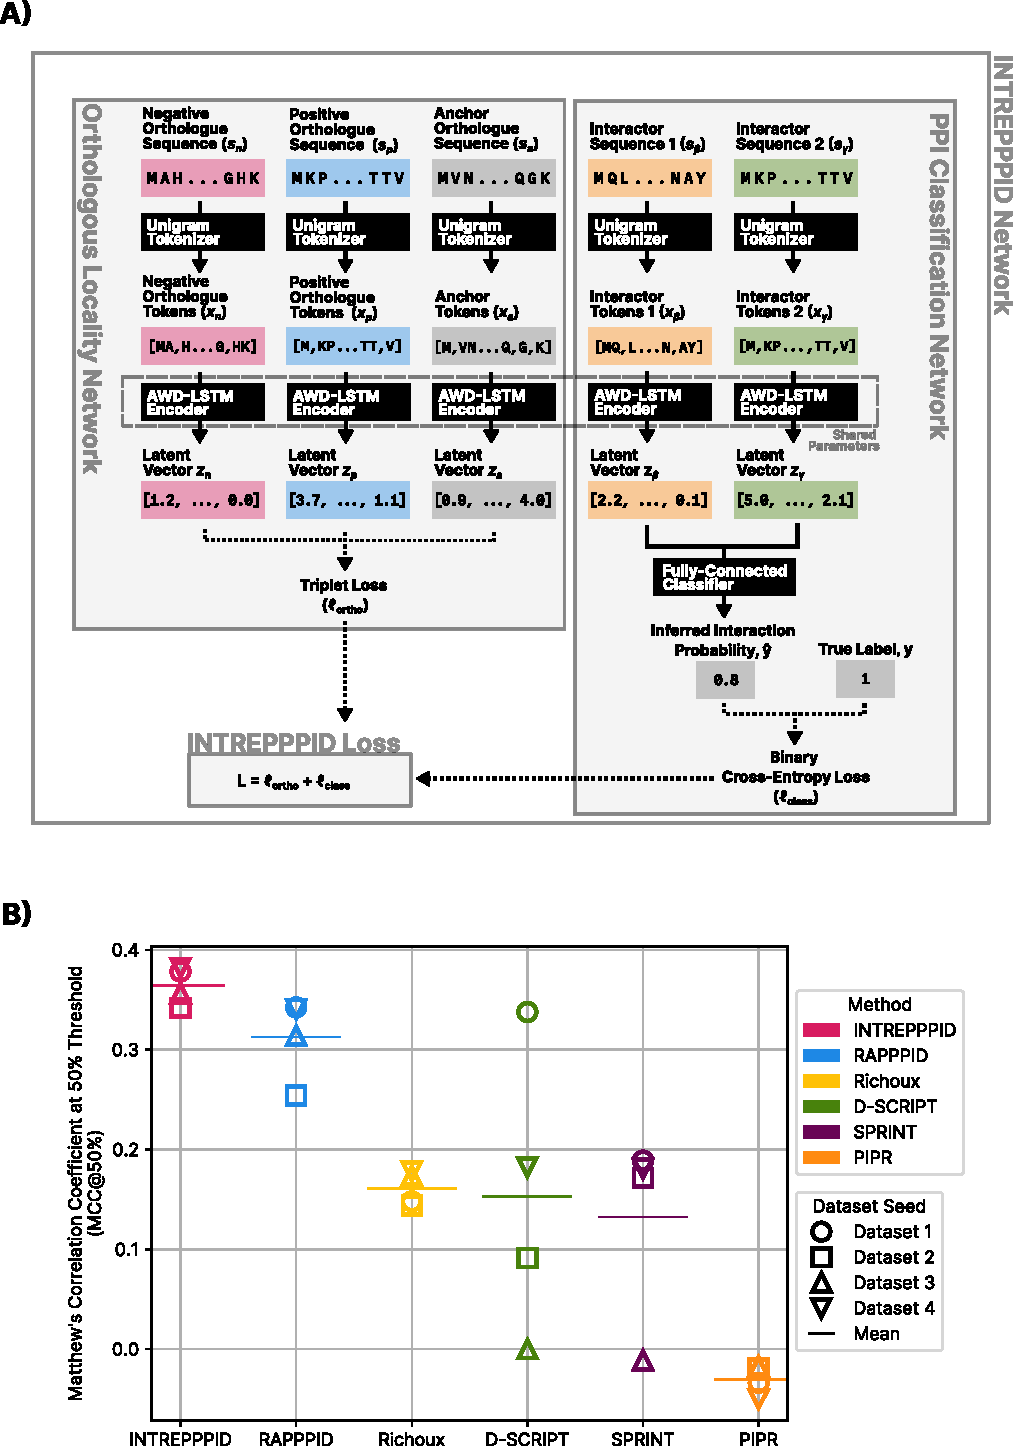
\includegraphics[scale=0.7]{figures/intrepppid/architecture_intra.pdf}
    }
    \caption[INTREPPPID’s architecture and performance.]{\textbf{\textsf{INTREPPPID’s architecture and performance.}} \textbf{(A)} A schematic overview of \textsc{intrepppid}’s quintuplet architecture. The leftmost panel depict s the triplet network responsible for the orthologous locality task, while the rightmost panel depicts the triplet network responsible for the \textsc{ppi} classification task. During training, \textsc{intrepppid} learns both tasks jointly through an overall loss function, which is the sum of the losses of the two tasks. \textbf{(B)} Test (\textsc{c3}) Matthew’s correlation coefficient (\textsc{mcc}) of leading \textsc{ppi} inference methods trained and tested on \textit{H.~sapiens} datasets.} \label{fig:intrepppid_architecture_intra}
\end{figure}

Unlike our benchmarks, it is estimated that there are far more pairs of proteins that do not interact than those that do [6, 42]. Accordingly, we tested \textsc{intrepppid}’s performance at increasing negative-to-positive interaction ratios and found that no appreciable change in performance was found (Supplementary Table \ref{tab:intrepppid_supp_neg_ratio}).

\begin{table}[!t]
    \label{tab:intrepppid_perf}
	\caption[Average performance of five leading \textsc{ppi} inference methods trained and tested on four \textit{H.~sapiens} \textsc{ppi} datasets.]{\textsf{\textbf{Average performance of five leading PPI inference methods trained and tested on four \textit{H.~sapiens} PPI datasets.}} The performance metrics are calculated on strict \textsc{c3} test sets (see \hyperref[sec:intrepppid_methods]{Materials and Methods}). The upward arrow (▲) indicates higher values are better for a metric, whereas a downward arrow (▼) indicates lower value are better. Boldface indicates the best value. The following abbreviations are used: \textsc{auroc}: area under the receiver operating characteristic; \textsc{ap}: average precision; \textsc{mcc}: Matthew’s correlation coefficient, \textsc{sd}: standard deviation. \label{tab:intrepppid_perf}} {\begin{tabular}{@{}lllllll@{}}\toprule 
			Method & INTREPPID & \textsc{rapppid} & \textsc{d-script} & Richoux \textit{et al.} & \textsc{sprint} & \textsc{pipr} \\\midrule
			▲ \textsc{auroc} & \textbf{0.752} & 0.732 & 0.634 & 0.606& 0.597& 0.482\\
            Mean (±\textsc{sd}) & (± 0.017) & (± 0.024) & (± 0.125) & (± 0.009)& (± 0.061)& (± 0.006)\\
            ▲ \textsc{ap} & \textbf{0.730} & 0.717 & 0.627 & 0.614& 0.641& 0.484\\
            Mean (±\textsc{sd}) & (± 0.022) & (± 0.015) & (± 0.086) & (± 0.015)& (± 0.064)& (± 0.003)\\
            ▲ \textsc{mcc}{@}50\% & \textbf{0.365} & 0.313 & 0.153 & 0.161& 0.133& -0.030\\
            Mean (±\textsc{sd}) & (± 0.067) & (± 0.041) & (± 0.144) & (± 0.017)& (± 0.096)& (± 0.015)\\
            ▲ $F_1${@}50\% & \textbf{0.697} & 0.630 & 0.506 & 0.370& 0.566& 0.318\\
            Mean (±\textsc{sd}) & (± 0.019) & (± 0.025) & (± 0.282) & (± 0.030)& (± 0.048)& (± 0.010)\\
            ▼ Brier Score & \textbf{0.200} & 0.215 & 0.402 & 0.274& 0.493& 0.487\\
            Mean (±\textsc{sd}) & (± 0.004) & (± 0.006) & (± 0.116) & (± 0.011)& (± 0.003)& (± 0.005)\\
			\midrule
	\end{tabular}}{}

\end{table}

\subsection*{INTREPPPID maintains high cross-species performance on multiple organisms}
\addcontentsline{toc}{subsection}{\textsc{intrepppid} maintains high cross-species performance on multiple organisms}

\textsc{intrepppid} was designed to improve on \textsc{rapppid}'s ability to make predictions across species. We therefore sought to compare \textsc{intrepppid}'s cross-species performance with that of \textsc{rapppid}'s as well as other leading \textsc{ppi} prediction methods.

When trained on \textit{H.~sapiens} and tested on various species (\textsc{c3}), ranging from \textit{Mus musculus} (house mouse) to \textit{Arabidopsis thaliana} (thale cress), \textsc{intrepppid} predominantly outperformed other methods (Fig. \ref{fig:intrepppid_cross_species}A, Supplementary Table \hyperref[sec:intrepppid_supp_s5]{S5}), with only \textsc{rapppid} rarely surpassing its performance in some metrics. Figure \ref{fig:intrepppid_cross_species}A shows the mean \textsc{auroc} (across three datasets) of different methods, with \textsc{intrepppid} significantly outperforming all other methods (one-sided Wilcoxon signed rank test versus \textsc{rapppid} = 0.03). On the cross-species task, the performance of \textsc{pipr} and \textsc{sprint} were close to a random classifier. Both \textsc{d-script} and the Richoux \textit{et al.} method performed similarly to one another, but consistently scored below \textsc{rapppid} and \textsc{intrepppid}.

In many applications, one is particularly interested in the precision of a model among the highest-ranking predicted edges (\textit{e.g.} to validate them experimentally). To evaluate \textsc{intrepppid}’s suitability for such tasks, we measured the precision of predictions whose scores are above various percentiles (Fig. \ref{fig:intrepppid_cross_species}B). Considering the average across all species tested, \textsc{intrepppid} achieved a precision $>90\%$ among predictions above the 85th percentile, and even when we considered the 75th percentile, its mean precision remained $>85\%$. These observations confirm that \textsc{intrepppid} is suitable for applications where very high precision is paramount.
\begin{figure}[h!]
	\centerline{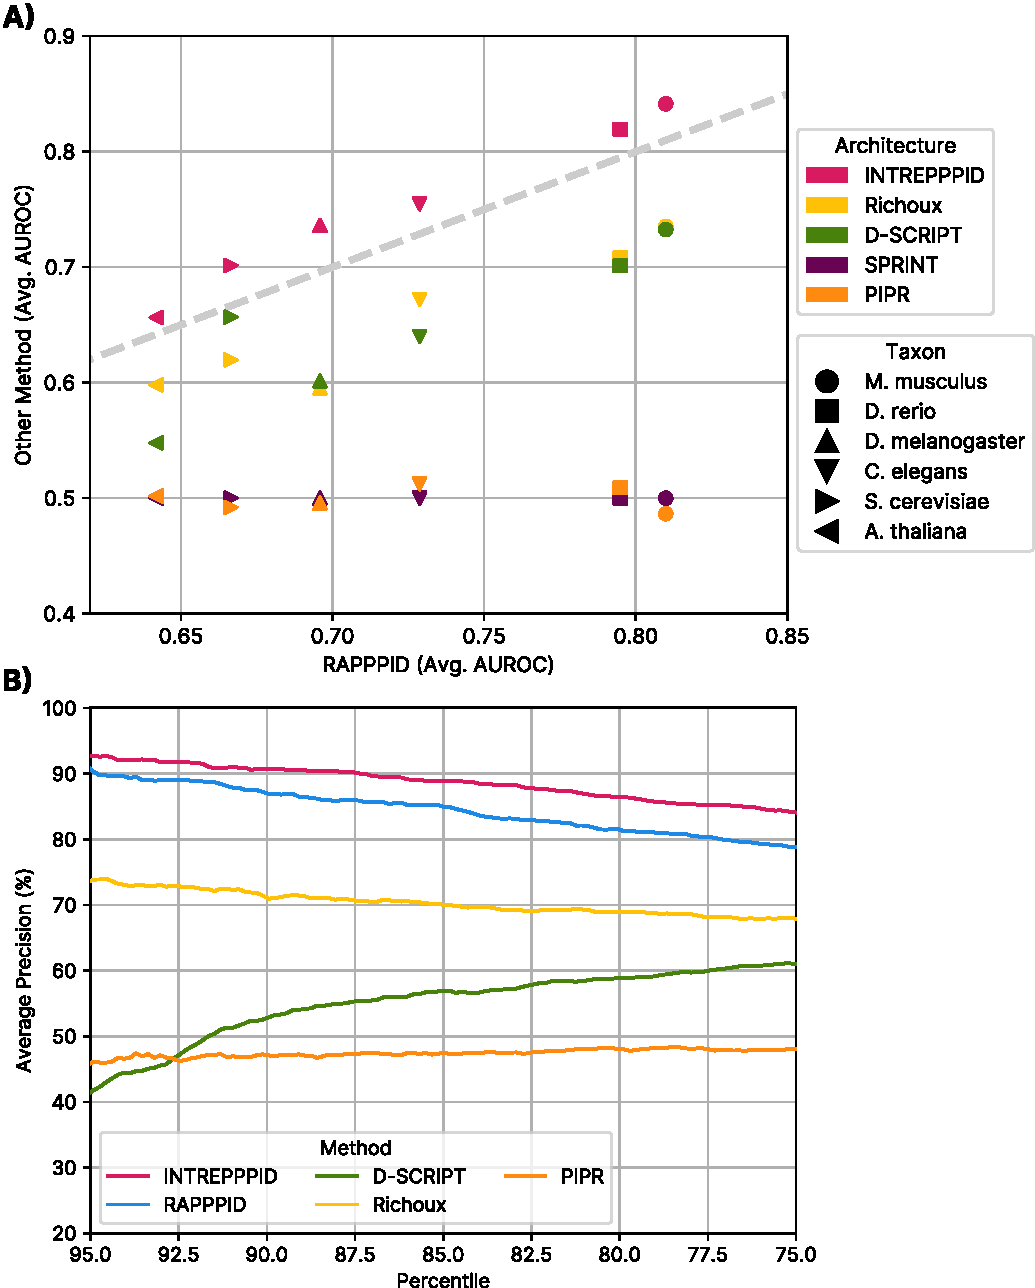
\includegraphics[scale=0.7]{figures/intrepppid/cross_species2.pdf}
    }
    \caption[Cross-species performance]{ \textbf{(A)} Average cross-species AUROC of leading \textsc{ppi} inference methods. The y-axis shows the \textsc{auroc} of each method (shown as different colours) against the \textsc{auroc} of \textsc{rapppid} (x-axis). Each model was trained on H.~sapiens and tested on various species (indicated by the different markers). Markers above the dashed grey line indicate instances where a method outperformed \textsc{rapppid}, while markers below the line indicate under-performance. \textbf{(B)} The precision of inferred interactions among the $k^\textrm{th}$ percentile of the scores inferred by the method indicated by the line colour. The x-axis shows $k$ and the y-axis shows precision along the y-axis. Interactions were inferred for datasets from seven different species. The mean across these datasets is reported by the solid line.}\label{fig:intrepppid_cross_species}
\end{figure}

We sought to further confirm \textsc{intrepppid}’s ability to generalize by measuring the number of interactions in additional \textsc{ppi} databases that \textsc{intrepppid} was capable of recovering. When considering interactions with confidence scores of 95\% or higher, \textsc{intrepppid} was capable of correctly identifying 72\% of interaction in the \textsc{hippie} database and 69\% of interaction in the IntAct database. These results are only slightly lower than the 74\% true-positive rate \textsc{intrepppid} achieves on our benchmark dataset.

\subsection*{INTREPPPID learns protein representations that exhibit strong orthologous locality}
\addcontentsline{toc}{subsection}{\textsc{intrepppid} learns protein representations that exhibit strong orthologous locality}
Through its orthologous locality task, \textsc{intrepppid} learns latent representations of orthologues that are near to one another in the Euclidean space, while ensuring latent representations of nonorthologous sequences remain distant. To qualitatively assess the locality of orthologues in latent space, we calculated the embeddings of the sequences of 1000 randomly sampled proteins present in the \textsc{oma} database of orthologues and projected them onto a \textsc{2d} space using \textsc{umap} and \textsc{pca} (Supplementary Fig. \ref{fig:intreppid_supp_scramble}) [43]. The projections show that embeddings of orthologues cluster tightly in \textsc{intrepppid}’s latent space, while embeddings from \textsc{rapppid} (which has a similar architecture, but without the triplet network) do not.

A more quantitative analysis of embedding distances further confirmed that \textsc{intrepppid}'s latent space exhibits strong orthologous locality. Namely, the Euclidean distance between latent representations of orthologues was on average 0.822, while the distance between the representations of nonorthologous proteins is on average 5.31 (Supplementary Fig. \ref{fig:intreppid_supp_scramble}C). Nearly 80\% of \textsc{intrepppid}'s latent representations of orthologues fell under the triplet loss margin of 1, while virtually all nonorthologues had a distance greater than the margin between them.

Together, these analyses confirm that \textsc{intrepppid} successfully accomplishes the orthologous locality task.

\subsection*{INTREPPPID's performance gain is due to the biologically relevant information encoded by orthology}
\addcontentsline{toc}{subsection}{\textsc{intrepppid}'s performance gain is due to the biologically relevant information encoded by orthology}

To further assess the role of orthology information on the performance of \textsc{intrepppid}, we conducted an experiment in which we trained \textsc{intrepppid} on two separate datasets: one constructed using orthologue data from the \textsc{oma} database (called `not scrambled') and one where `random' pairs of proteins from the \textsc{oma} database were labelled orthologues (`scrambled'). After training and testing on both variants of the \textit{H.~sapiens} dataset, we found that \textsc{intrepppid}’s performance dropped to near random in the `scrambled' case (Supplementary Table \ref{tab:intrepppid_supp_scramble}, \textsc{auroc} = 0.524). Moreover, on this dataset, neither the classification loss nor the triplet loss significantly changed over 30~000 training steps (Supplementary Fig. \ref{fig:intreppid_supp_scramble}D).

\textsc{intrepppid}'s low testing performance on `scrambled' data suggests that the mere exposure of sequences from various species is not sufficient to increase \textsc{ppi} classification performance. The impact of the `scramble' dataset on both the classification and triplet losses suggests that the orthologous locality task is complimentary to the \textsc{ppi} classification task. Ablating the biological meaning of the orthology data conversely results in the orthologous locality task negatively impacting \textsc{ppi} classification performance. These results show that the encoding of orthology information increases \textsc{intrepppid}'s performance due to its biological relevance.

Having established that the central contribution of incorporating orthologues in the \textsc{intrepppid} model is the biological information they encode, we continued to test the extent to which they are relevant to \textsc{intrepppid}'s performance. To do so, we constructed \textsc{intrepppid} datasets of \textit{H.~sapiens} protein interactions much as we have for previous cross-species analyses herein. For this analysis, however, orthology data related to proteins belonging to any of the testing species (\textit{H.~sapiens}, \textit{M.~musculus}, \textit{Danio rerio}, \textit{Drosophila melanogaster}, \textit{Caenorhabditis elegans}, \textit{Saccharomyces cerevisiae}, \textit{A.~thaliana}) were omitted. Relative to \textsc{intrepppid} trained on dataset that included all available orthology data, the altered dataset resulted in worse testing performance metrics across every species tested (Supplementary Table \ref{tab:intrepppid_supp_no_ortho}). The decrease in performance was least severe when testing on \textit{H.~sapiens} (\textit{i.e.} intraspecies inference), having measured a $−9.00\%$ change in \textsc{mcc} and $−1.36\%$ change in \textsc{ap} scores. Conversely, the performance drop was much greater on testing sets of species different from the training species (\textit{i.e.} cross-species inference), with observed changes as low as $−38.85\%$ for \textsc{mcc} and $-17.58\%$ for \textsc{ap} scores in some instances. This further confirms that orthology information is used by the model to make predictions.

\subsection*{INTREPPPID learns interactions of evolutionarily conserved functions that RAPPPID does not}
\addcontentsline{toc}{subsection}{\textsc{intrepppid} learns interactions of evolutionarily conserved functions that \textsc{rapppid} does not}

To better understand the biological characteristics of the interactions that account for \textsc{intrepppid}’s performance gains and the role that its orthology loss plays, we analysed the pairs of interacting proteins from our testing datasets in which \textsc{intrepppid} predicted a higher probability of interaction than \textsc{rapppid} by the widest margin. We found that, on average, \textsc{intrepppid} assigns higher scores to interacting pairs in 73\% ($\pm11\%$) of all cases. Of those inferred interactions, the top interactions were disproportionately between proteins that are evolutionarily conserved between species.

Our analysis began with pairs of proteins in the testing dataset that interact and were correctly identified by \textsc{intrepppid} (\textit{i.e.} a score $\geq0.5$), and incorrectly identified by \textsc{rapppid} (\textit{i.e.} a score $<0.5$). To examine cases in which most typified \textsc{intrepppid} are performing well while \textsc{rapppid} are falling short, we further filtered the aforementioned interactions such that only protein pairs with the largest differences between the \textsc{intrepppid} and \textsc{rapppid} scores remained (\textit{i.e.} in the 90th percentile or higher). These scored protein pairs will be referred to as `top \textsc{intrepppid} unique positive hits' hereafter.

A statistical analysis of over-representation of Gene Ontology (\textsc{go}) Molecular Function annotations was performed on the top \textsc{intrepppid}-unique positive hits using the \textsc{panther} Classification System [44–46]. This analysis provided us with an understanding of which \textsc{go} Molecular Function annotations were over-represented among proteins that comprised the top \textsc{intrepppid}-unique positive hits, relative to those in the testing set as a whole.

We found that, across the species tested, the \textsc{go} Molecular Function annotations that were overexpressed were primarily regarding ubiquinone activity, ribosome structure, and \textsc{rna} binding (Supplementary Table \hyperref[sec:intrepppid_supp_s8]{S8}). These functions all belong to pathways that are consistently found to be highly conserved across a broad spectrum of species [18, 47, 48].

An example of one of these interactions is one between the large ribosomal subunit proteins uL24A and uL10 found in \textit{S. cerevisiae} encoded by the genes \textit{RPL26A} and \textit{RPP0}, respectively. \textsc{intrepppid} correctly predicts that these two proteins interact with a probability of 94.6\% while \textsc{rapppid} assigns a probability of 4.52\%, both models having been trained exclusively on interactions between human proteins. The two proteins in question are highly conserved, with 131 and 798 orthologues recorded in the \textsc{oma} database for each protein, respectively. In both cases, a human orthologue is identified by \textsc{oma} (\textit{RPL26L1} and \textit{RPLP0} genes, respectively).

These observations suggests that \textsc{intrepppid} correctly identifies interactions that have functions crucial to pathways such as protein degradation and protein translation that are highly conserved between species, that \textsc{rapppid} does not. In addition, these observations provide further support that the discrepancy between \textsc{intrepppid} and \textsc{rapppid}’s performance among interactions composed of highly conserved proteins is driven by the similarity of embeddings among orthologous proteins (\textit{i.e.} the orthologous locality property), which is the primary distinction between \textsc{intrepppid} and \textsc{rapppid}.

\subsection*{A web server and interface for RAPPPID \& INTREPPPID}
\addcontentsline{toc}{subsection}{A web server and interface for \textsc{rapppid} \& \textsc{intrepppid}}
While we have made best efforts to make \textsc{rapppid} and \textsc{intrepppid} as simple as possible to run on a local computer with minimal computational requirements, it currently requires knowledge of the \textsc{cli} and the Python computer language. These prerequisites, while accessible to researchers with relevant experience, can be too great a hurdle for others.

To address this, we have created a website which acts as a graphical interface for a server that is capable of performing proteome-scale inference in under 15 min (\href{https://ppi.bio}{https://ppi.bio}). The source code that runs \textsc{ppi}.bio is available publicly on GitHub and can be found by visiting the internet address: \href{https:// github.com/Emad-COMBINE-lab/ppi.bio}{https:// github.com/Emad-COMBINE-lab/ppi.bio}. Many online academic servers are no longer available online and do not provide their source openly, resulting in the total loss of these servers (see Supplementary Table \ref{tab:intrepppid_supp_links} for a review of 22 such resources, 50\% of which are no longer alive). We hope to enable others to run their own server in the event that \href{https://ppi.bio}{https://ppi.bio} goes off line by releasing its code and documentation.

\begin{figure}[h!]
	\centerline{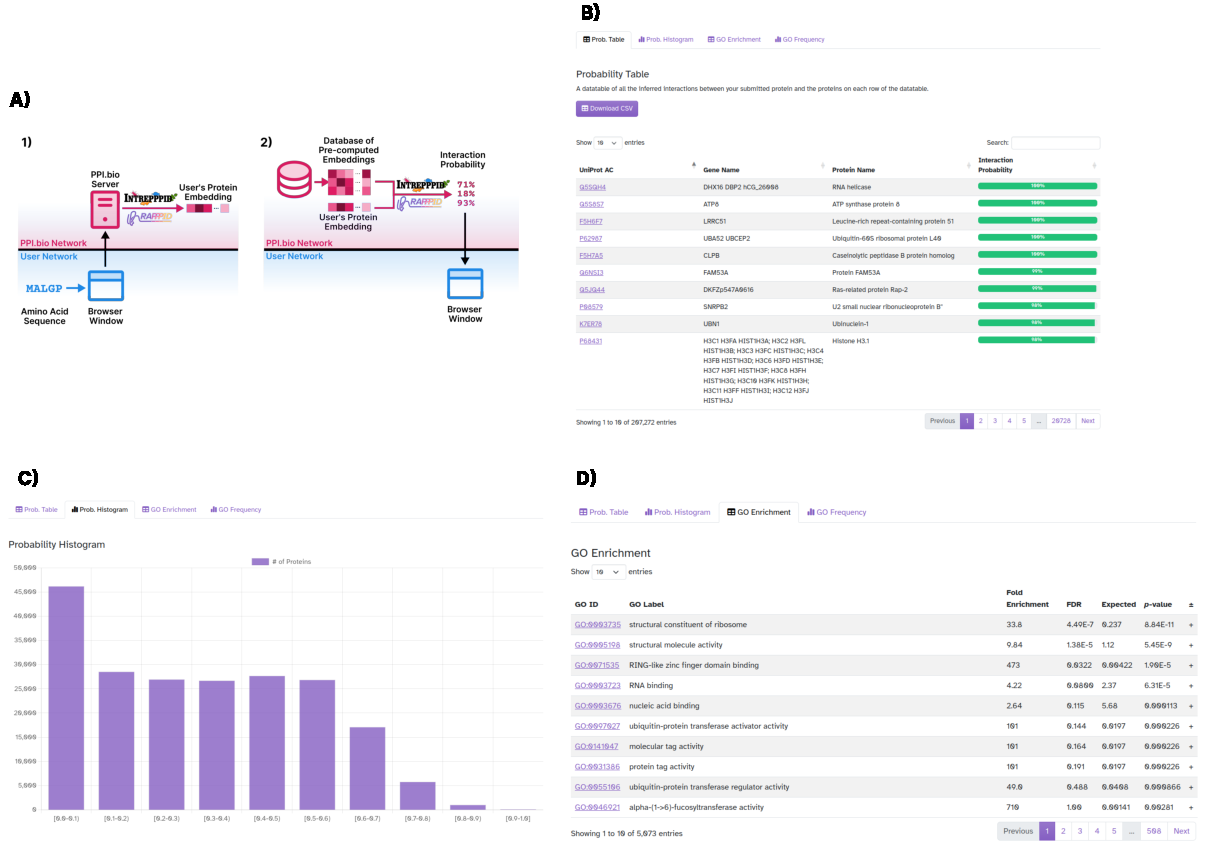
\includegraphics[scale=0.7]{figures/intrepppid/ppibio_screens.pdf}
    }
    \caption[The webserver of \textsc{ppi}.Bio supporting \textsc{rapppid} and \textsc{intrepppid} at whole proteome scale.]{\textbf{\textsf{The webserver of PPI.Bio supporting RAPPPID and INTREPPPID at whole proteome scale.}} \textbf{(A)} Overview of the operation of the \textsc{ppi}.Bio \textsc{ppi} inference server. In the first stage (leftmost panel), amino acid sequences are encoded into protein embeddings using either \textsc{rapppid} or \textsc{intrepppid}, depending on the user’s preference. In the second stage (rightmost panel), precomputed protein embeddings of a specified species proteome are loaded from a database. The classification head of either \textsc{rapppid} or \textsc{intrepppid} is then used to compute the probability of interaction of the user-specified protein and the precomputed embeddings. Screenshot of the \textbf{(B)} data table of interaction probabilities, \textbf{(C)} probability histograms, and \textbf{(D)} \textsc{go} enrichment analysis powered by \textsc{pantherdb}, as seen on \textsc{ppi}.Bio after inferring proteome-wide interactions.}\label{fig:intrepppid_ppi_bio}
\end{figure}

The process for making proteome-wide inferences on user-submitted amino acid sequence is as follows. Users input amino acid sequences that are then submitted to the \textsc{ppi}.bio server (Fig. \ref{fig:intrepppid_ppi_bio}). The \textsc{ppi}.bio server in turn encodes the sequence using the user’s choice of either \textsc{rapppid} or \textsc{intrepppid}’s encoder to obtain a protein embedding. The embedding is then paired with precomputed embeddings of all proteins belonging to the proteome of the user’s choosing (currently, proteins for six organisms have been computed). The probability of these pairs of proteins interacting are then inferred using \textsc{rapppid} or \textsc{intrepppid}’s classification head (based on the user’s choice), and returned to the user’s browser window.

\textsc{ppi}.bio also enables users to conduct \textsc{go} enrichment analysis on the set of proteins that have an interaction probability greater than some user-specified threshold. \textsc{ppi}.bio uses the \textsc{panther} online \textsc{api} [44] to calculate \textsc{go} enrichment statistics. This functionality allows users to find instances of \textsc{go} annotations being statistically over-represented among proteins that were inferred to interact with the protein supplied by the user.

\section*{Discussion}
\addcontentsline{toc}{section}{Discussion}
This study introduces three tools for researchers in their pursuit of better understanding \textsc{ppi}s: a cross-species method for \textsc{ppi} inference (\textsc{intrepppid}), a software package for creating strict \textsc{ppi} datasets (\textsc{ppi} Origami), and a web server for inferring \textsc{ppi}s using \textsc{intrepppid} and \textsc{rapppid} (\textsc{ppi}.bio). These tools and their code are all freely available under open licenses with complete documentation.

We view \textsc{intrepppid}’s novel contributions as being two-fold. First, \textsc{intrepppid} is among the few sequence-based \textsc{ppi} inference methods that are specifically designed with the purpose of addressing the challenge of accurately inferring protein interactions between proteins of species other than that it was trained on (\textit{i.e.} cross-species inference). The only other such methods specifically designed for this purpose known to us are \textsc{d-script} and \textsc{pipe4} [40, 49]. Of these two methods, only \textsc{d-script}’s software is made publicly available, which has made its inclusion in the analyses herein possible. We believe that \textsc{intrepppid} joining \textsc{d-script} in being the only publicly available sequence-based cross-species \textsc{ppi} inference methods represents a significant contribution to the community.

Secondly, \textsc{intrepppid} introduces a novel orthologous locality loss and quintuplet architecture which, as we demonstrated, is responsible for a significant increase in both intra- and crosss-pecies \textsc{ppi} inference performance under strict evaluation conditions. While \textsc{intrepppid} has a quintuplet network, there is no appreciable increase in trainable parameters compared to \textsc{rapppid}’s twin network construction due to the parameter sharing between encoders (2.20E5 and 1.88E5 parameters, respectively). By sharing parameters, \textsc{intrepppid} reduces both its \textsc{gpu} memory footprint as well as the risk of over-fitting via over-parameterization.

The orthologous locality task can be viewed through the lens of contrastive self-supervised learning (\textsc{ssl}) techniques like ‘Sim\textsc{clr}’ or Time-Contrastive Networks [50, 51]. Specifically, orthologous sequences can be thought of as multiple views of the same protein augmented by an evolutionary process in a way that is analogous to how Sim\textsc{clr} compares pairs of images that have been augmented by, \textit{e.g.} cropping or blurring. In both instances, the model is learning invariance between entities that are similar in their desired feature space, but are significantly different in the input space. By creating a feature space that is invariant to the effects of speciation on amino acid sequences, we position our model to capture more interologues. While Sim\textsc{clr} only uses pairs of contrasting examples, \textsc{ssl} methods like time-contrastive networks have adopted a triplet loss to more efficiently learn embeddings that better fit downstream tasks.

Sequence-based methods rely on a large number of \textsc{ppi} examples to learn to recognize features in pairs of amino acid sequences that indicate two pairs of proteins are likely to interact. The more examples provided, the better models become at identifying features that we know from experimental knowledge are important for mediating interactions.

As is the case with all sequence-based methods for \textsc{ppi} inference, \textsc{intrepppid} risks becoming brittle and only memorizing sequences found in the training set or learning trivial solutions such as reporting the sequence similarity of two proteins as their likelihood of interaction. In the absence of more experimental data to train on, ensuring the data are of high-quality, validating strictly and judicious application of regularization are the primary ways to address these generalization concerns. Our previous work on \textsc{rapppid} underscores how these methods can be used to create generalized, performant models that do not rely on trivial solutions like comparing sequence similarity nor memorizing sequences.

While \textsc{intrepppid} is shown here to outperform leading methods in the intra- and cross-species tasks, it is important to note that deep learning, sequence-based methods like ours can sometimes struggle with the changes observed by certain protein variants and isoforms. Future work might help address this by constructing architectures that provide inductive biases relevant to learning binding domains and residues.

Additionally, all of the sequence-based methods tested infer interactions that occur under unspecified intrinsic (\textit{e.g.} protein conformation, post-translational modifications) and extrinsic (\textit{e.g.} subcellular localization, p\textsc{h}, temperature) conditions (a property inherited from the training \textsc{string} dataset). While databases such as Reactome richly annotate interactions, including information about, \textit{e.g.} \textsc{ptm}s and subcellular localizations, the number of interactions and organisms in the database is limited due to the high-labour costs associated with manual curation [52]. Future work towards reconciling and augmenting existing \textsc{ppi} datasets and methods with such annotations could possibly help to provide valuable context to the interactions provided.

The second tool presented in this work is \textsc{ppi} Origami, a framework for creating new strict \textsc{ppi} datasets. While many reference or `gold-standard' \textsc{ppi} datasets exist, they each bring with them different underlying assumptions and limitations [11–13]. Researchers might wish to take advantage of large, comprehensive \textsc{ppi} databases like the \textsc{string} database used to create the aforementioned strict \textsc{ppi} datasets or alternatively take a specialist approach and interrogate smaller curated networks that describe certain organisms, diseases, or cell types [53–55]. They may also wish to derive their training set from one dataset and their evaluation datasets from another, much as we did over the course of our experiments. \textsc{ppi} Origami provides tools for creating \textsc{ppi} datasets from sources the user specifies, while automating the process of ensuring that the data conform to the criteria outlined herein. By providing tools and frameworks rather than one set of datasets, we hope to impower researchers to adopt \textsc{ppi} datasets that (i) do not leak data and (ii) conform to the specific needs of the researcher.

The final major contribution herein is \textsc{ppi}.bio, a web server for inferring \textsc{ppi}s using \textsc{rapppid} and \textsc{intrepppid}. \textsc{ppi}.bio infers interactions entirely on the Central Processing Unit (\textsc{cpu}), greatly reducing server costs. Both \textsc{rapppid} and \textsc{intrepppid} facilitate this by allowing known protein sequences to be precomputed, only requiring a forward pass of the shallow fully connected classification network when the embeddings for both proteins has already been calculated. This allows for significant speed-ups when doing proteome-wide inferences.

As time passes, online services published in academic articles tend to go off line or otherwise become inaccessible. After conducting a search for the terms `protein-protein interaction portal' and `protein-protein interaction website' on the online academic search engine SemanticScholar.org and randomly sampling 22 articles that introduce online tools, 45\% of the \textsc{uri}s either did not resolve or no longer offered the service introduced (Supplementary Table \ref{tab:intrepppid_supp_links}). To help ensure that \textsc{ppi}.bio remains accessible for years to come, we’ve made the code that runs \textsc{ppi}. bio available under a free and open license. To help facilitate the deployment of \textsc{ppi}.bio, the server is designed to be easily deployed to the Platform as a Service (\textsc{p}aa\textsc{s}) service Heroku as well as the self-hosted alternative Dokku.

\section*{Key Points}
\begin{itemize}
    \item Most \textsc{ppi} studies are conducted in a select few organisms, leading to a `species gap'.
    \item Performant cross-species \textsc{ppi} methods are required to bridge this species gap.
    \item We introduce \textsc{intrepppid}, which improves cross-species performance using a novel quintuplet architecture to incorporate orthology data.
    \item \textsc{intrepppid} outperforms leading \textsc{ppi} inference methods on both intra and cross-species tasks across multiple metrics.
    \item We also have released an online interface for \textsc{intrepppid} (\textsc{ppi}.bio) and a tool for making \textsc{ppi} datasets (\textsc{ppi} Origami).
\end{itemize}

\section*{Supplementary data}
\href{https://academic.oup.com/bib/article-lookup/doi/10.1093/bib/bbae405#supplementary-data}{Supplementary data} are available at \textit{Briefings in Bioinformatics} online.

\section*{Author contributions}
\addcontentsline{toc}{section}{Author contributions}

\textsc{a.e.} and \textsc{j.s.} contributed to project conceptualization, methodology as well as writing, editing, and reviewing. \textsc{a.e.} contributed to supervision and funding acquisition. \textsc{j.s.} contributed to software, data curation, investigation and visualization. All authors read and approved the final article.

\section*{Funding}
\addcontentsline{toc}{section}{Funding}
This work was supported by grants from Natural Sciences and Engineering Research Council of Canada (\textsc{nserc}) [\textsc{rgpin}-201904460] (\textsc{a.e.}) and Canada Foundation for Innovation (\textsc{cfi}) \textsc{jelf} [project 40781]. This research was enabled in part by support provided by Calcul Québec (www.calculquebec.ca) and the Digital Research Alliance of Canada (alliancecan.ca).

\section*{Software \& data availability}
\textsc{intrepppid} and the \textsc{ppi}.bio server are freely available under the Affero General Public License version 3.0. \textsc{ppi} Origami is licensed under the \textsc{gnu} General Public License version 3.0. They can be downloaded from \href{https://github.com/Emad-COMBINE-lab/intrepppid}{https://github.com/Emad-COMBINE-lab/intrepppid},\\\href{https://github.com/Emad-COMBINE-lab/ppi.bio}{https://github.com/Emad-COMBINE-lab/ppi.bio}, and \href{https://github.com/Emad-COMBINE-lab/ppi_origami}{https://github.com/Emad-COMBINE-lab/ppi\_origami}, respectively. All code and datasets have been deposited in the Zenodo repository under record numbers \href{https://zenodo.org/doi/10.5281/zenodo.10652231}{10652231}, \href{https://zenodo.org/doi/10.5281/zenodo.10652229}{10652229}, \href{https://zenodo.org/doi/10.5281/zenodo.10652233}{10652233}, and \href{https://zenodo.org/doi/10.5281/zenodo.10594149}{10594149}.

\section*{References}
\addcontentsline{toc}{section}{References}

\begin{singlespace}
\begin{enumerate}
    \item Cheng F, Zhao J, Wang Y, \textit{et al.} Comprehensive characterization of protein–protein interactions perturbed by disease mutations. \textit{Nat Genet} 2021;\textbf{53}:342–53. \\\href{https://doi.org/10.1038/s41588-020-00774-y}{https://doi.org/10.1038/s41588-020-00774-y}.
    \item Richards AL, Eckhardt M, Krogan NJ. Mass spectrometry-based protein–protein interaction networks for the study of human diseases. \textit{Mol Syst Biol} 2021;\textbf{17}:e8792. \\\href{https://doi.org/10.15252/msb.20188792}{https://doi.org/10.15252/msb.20188792}.
    \item Gordon DE, Jang GM, Bouhaddou M, \textit{et al.} A SARS-CoV-2 protein interaction map reveals targets for drug repurposing. \textit{Nature} 2020;583:459–68. \\\href{https://doi.org/10.1038/s41586-020-2286-9}{https://doi.org/10.1038/s41586-020-2286-9}.
    \item Mabonga L, Kappo AP. Protein-protein interaction modulators: advances, successes and remaining challenges. \textit{Biophys Rev} 2019;11:559–81. \\\href{https://doi.org/10.1007/s12551-019-00570-x}{https://doi.org/10.1007/s12551-019-00570-x}.
    \item Rolland T, Taşan M, Charloteaux B, \textit{et al.} A proteome-scale map of the human Interactome network. \textit{Cell} 2014;159:1212–26. \\\href{https://doi.org/10.1016/j.cell.2014.10.050}{https://doi.org/10.1016/j.cell.2014.10.050}.
    \item Luck K, Kim D-K, Lambourne L, \textit{et al.} A reference map of the human binary protein interactome. \textit{Nature} 2020;580:402–8.  \\\href{https://doi.org/10.1038/s41586-020-2188-x}{https://doi.org/10.1038/s41586-020-2188-x}.
    \item Schoch CL, Ciufo S, Domrachev M, \textit{et al.} NCBI taxonomy: a comprehensive update on curation, resources and tools. \textit{Database} 2020;\textbf{2020}:baaa062. \\\href{https://doi.org/10.1093/database/baaa062}{https://doi.org/10.1093/database/baaa062}.
    \item Szklarczyk D, Kirsch R, Koutrouli M, \textit{et al.} The STRING database in 2023: protein–protein association networks and functional enrichment analyses for any sequenced genome of interest. \textit{Nucleic Acids Res} 2023;\textbf{51}:D638–46. \\\href{https://doi.org/10.1093/nar/gkac1000}{https://doi.org/10.1093/nar/gkac1000}.
    \item International commission on zoological nomenclature. \textit{International code of zoological nomenclature} 1999;\textbf{1999}:1–344.
    \item Low TY, Syafruddin SE, Mohtar MA, \textit{et al.} Recent progress in mass spectrometry-based strategies for elucidating protein-protein interactions. Cell \textit{Mol Life Sci} 2021;\textbf{78}:5325–39. \\\href{https://doi.org/10.1007/s00018-021-03856-0}{https://doi.org/10.1007/s00018-021-03856-0}.
    \item Park Y, Marcotte EM. Flaws in evaluation schemes for pair-input computational predictions. \textit{Nat Methods} 2012;\textbf{9}:1134–6. \\\href{https://doi.org/10.1038/nmeth.2259}{https://doi.org/10.1038/nmeth.2259}.
    \item Dunham B, Ganapathiraju MK. Benchmark evaluation of protein–protein interaction prediction algorithms. \textit{Molecules} 2021;\textbf{27}:41. \\\href{https://doi.org/10.3390/molecules27010041}{https://doi.org/10.3390/molecules27010041}.
    \item Bernett J, Blumenthal DB, List M. Cracking the black box of deep sequence-based protein-protein interaction prediction. \textit{Briefings in Bioinformatics} 2024;\textbf{25}:bbae076. \\\href{https://doi.org/10.1093/bib/bbae076}{https://doi.org/10.1093/bib/bbae076}.
    \item Hamp T, Rost B. More challenges for machine-learning protein interactions. \textit{Bioinformatics} 2015;31:1521–5. \\\href{https://doi.org/10.1093/bioinformatics/btu857}{https://doi.org/10.1093/bioinformatics/btu857}.
    \item Marcotte EM, Pellegrini M, Ng H-L, \textit{et al.} Detecting protein function and protein-protein interactions from genome sequences. Science 1999;285:751–3. https://doi.org/10.1126/ science.285.5428.751.
    \item Walhout AJM, Sordella R, Lu X, \textit{et al.} Protein interaction mapping in C. Elegans using proteins involved in Vulval development. \textit{Science} 2000;\textbf{287}:116–22. \\\href{https://doi.org/10.1126/science.287.5450.116}{https://doi.org/10.1126/science.287.5450.116}.
    \item Matthews LR, Vaglio P, Reboul J, \textit{et al.} Identification of potential interaction networks using sequence-based searches for conserved protein-protein interactions or ‘interologs’. \textit{Genome Res} 2001;\textbf{11}:2120–6. \\\href{https://doi.org/10.1101/gr.205301}{https://doi.org/10.1101/gr.205301}.
    \item Sharan R, Suthram S, Kelley RM, \textit{et al.} Conserved patterns of protein interaction in multiple species. \textit{Proc Natl Acad Sci} 2005;\textbf{102}: 1974–9. \\\href{https://doi.org/10.1073/pnas.0409522102}{https://doi.org/10.1073/pnas.0409522102}.
    \item Cortes C, Vapnik V. Support-vector networks. \textit{Mach Learn} 1995;20:273–97. \\\href{https://doi.org/10.1007/BF00994018}{https://doi.org/10.1007/BF00994018}.
    \item Ben-Hur A, Noble WS. Kernel methods for predicting proteinprotein interactions. \textit{Bioinformatics} 2005;\textbf{21}:i38–46. \\\href{https://doi.org/10.1093/bioinformatics/bti1016}{https://doi.org/10.1093/bioinformatics/bti1016}.
    \item Richoux F, Servantie C, Borès C, \textit{et al.} Comparing two deep learning sequence-based models for protein-protein interaction prediction. \textit{arXiv:190106268 [cs, q-bio, stat]} 2019.
    \item Bromley J, Bentz JW, Bottou L, \textit{et al.} Signature verification using a ``siamese'' time delay neural network. \textit{Int J Patt Recogn Artif Intell} 1993;\textbf{07}:669–88. \\\href{https://doi.org/10.1142/S0218001493000339}{https://doi.org/10.1142/S0218001493000339}.
    \item Baldi P, Chauvin Y. Neural networks for fingerprint recognition. \textit{Neural Comput} 1993;\textbf{5}:402–18. \\\href{https://doi.org/10.1162/ neco.1993.5.3.402}{https://doi.org/10.1162/ neco.1993.5.3.402}.
    \item Koch G, Zemel R, Salakhutdinov R. Siamese Neural Networks for One-shot Image Recognition. \textit{Proceedings of the 32nd International Conference on Machine Learning}. Lille, France, 2015;\textbf{37}.
    \item Chen M, Ju CJ-T, Zhou G, \textit{et al.} Multifaceted protein–protein interaction prediction based on Siamese residual RCNN. \textit{Bioinformatics} 2019;\textbf{35}:i305–14. \\\href{https://doi.org/10.1093/bioinformatics/btz328}{https://doi.org/10.1093/bioinformatics/btz328}.
    \item Cho K, van Merrienboer B, Gulcehre C. \textit{et al.} Learning Phrase Representations using RNN Encoder-Decoder for Statistical Machine Translation. \textit{arXiv:1406.1078 [cs.CL]} 2014.
    \item Szymborski J, Emad A. RAPPPID: towards generalizable protein interaction prediction with AWD-LSTM twin networks. \textit{Bioinformatics} 2022;\textbf{38}:3958–67. \\\href{https://doi.org/10.1093/bioinformatics/btac429}{https://doi.org/10.1093/bioinformatics/btac429}.
    \item Merity S, Keskar NS, Socher R. Regularizing and optimizing LSTM language models. \textit{arXiv:170802182 [cs]} 2017.
    \item Kudo T, Richardson J. SentencePiece: A simple and language independent subword tokenizer and detokenizer for Neural Text Processing. In: Blanco E, Lu W (eds), \textit{Proceedings of the 2018 Conference on Empirical Methods in Natural Language Processing: System Demonstrations.} Brussels, Belgium: Association for Computational Linguistics, 2018;66–71.
    \item Kudo T. Subword regularization: improving neural network translation models with multiple subword candidates. \textit{arXiv:180410959 [cs]} 2018.
    \item Misra D. Mish: a self regularized non-monotonic activation function. \textit{arXiv:190808681 [cs, stat]} 2020.
    \item Zhang X, Yu FX, Kumar S, \textit{et al.} Learning Spread-Out Local Feature Descriptors. 2017 \textit{IEEE International Conference on Computer Vision (ICCV)}. Venice, Italy: IEEE, \textbf{2017};4605–13.
    \item Altenhoff AM, Train C-M, Gilbert KJ, \textit{et al.} OMA orthology in 2021: website overhaul, conserved isoforms, ancestral gene order and more. \textit{Nucleic Acids Res} 2021;\textbf{49}:D373–9. \\\href{https://doi.org/10.1093/nar/gkaa1007}{https://doi.org/10.1093/nar/gkaa1007}.
    \item Schroff F, Kalenichenko D, Philbin J. FaceNet: a unified embedding for face recognition and clustering. 2015 \textit{IEEE Conference on Computer Vision and Pattern Recognition (CVPR)} 2015;815–23.
    \item Forslund K. \textit{The relationship between orthology, protein domain architecture and protein function.} Sweden: University of Stockholm in Stockholm, 2011.
    \item Fang G, Bhardwaj N, Robilotto R, \textit{et al.} Getting started in gene Orthology and functional analysis. \textit{PLoS Comput Biol} 2010;\textbf{6}:1–8. \\\href{https://doi.org/10.1371/journal.pcbi.1000703}{https://doi.org/10.1371/journal.pcbi.1000703}.
    \item Wright L, Demeure N. Ranger21: a synergistic deep learning optimizer, \textit{arXiv:2106.13731 [cs.LG]} 2021. \\\href{http://arxiv.org/abs/2106.13731}{http://arxiv.org/abs/2106.13731}.
    \item Loshchilov I, Hutter F. Decoupled Weight Decay Regularization. \textit{7th International Conference on Learning Representations} 2019.
    \item Iyer N, Thejas V, Kwatra N. \textit{et al.} Wide-minima Density Hypothesis and the Explore-Exploit Learning Rate Schedule \textit{arXiv:2003.03977 [cs.LG]} 2021.
    \item Sledzieski S, Singh R, Cowen L, \textit{et al.} D-SCRIPT translates genome to phenome with sequence-based, structure-aware, genome-scale predictions of protein-protein interactions. cels 2021;\textbf{12}:969–982.e6. \\\href{https://doi.org/10.1016/j.cels.2021.08.010}{https://doi.org/10.1016/j.cels.2021.08.010}.
    \item Li Y, Ilie L. SPRINT: ultrafast protein-protein interaction prediction of the entire human interactome. \textit{BMC Bioinformatics} 2017;\textbf{18}:485. \\\href{https://doi.org/10.1186/s12859-017-1871-x}{https://doi.org/10.1186/s12859-017-1871-x}.
    \item Venkatesan K, Rual J-F, Vazquez A, \textit{et al.} An empirical framework for binary interactome mapping. Nat Methods 2009;\textbf{6}:83–90. \\\href{https://doi.org/10.1038/nmeth.1280}{https://doi.org/10.1038/nmeth.1280}.
    \item McInnes L, Healy J, Melville J. UMAP: Uniform Manifold Approximation and Projection for Dimension Reduction \textit{arXiv:1802.03426 [stat.ML]} 2020.
    \item Thomas PD, Ebert D, Muruganujan A, \textit{et al.} PANTHER: making genome-scale phylogenetics accessible to all. Protein Sci 2022;\textbf{31}: 8–22. \\\href{https://doi.org/10.1002/pro.4218}{https://doi.org/10.1002/pro.4218}.
    \item Mi H, Muruganujan A, Huang X, \textit{et al.} Protocol update for large-scale genome and gene function analysis with PANTHER classification system (v.14.0). \textit{Nat Protoc} 2019;\textbf{14}:703–21. \\\href{https://doi.org/10.1038/s41596-019-0128-8}{https://doi.org/10.1038/s41596-019-0128-8}.
    \item The Gene Ontology Consortium, Aleksander SA, Balhoff J, \textit{et al.} The gene ontology knowledgebase in 2023. \textit{Genetics} 2023;\textbf{224}:iyad031. \\\href{https://doi.org/10.1093/genetics/iyad031}{https://doi.org/10.1093/genetics/iyad031}.
    \item Kelley BP, Sharan R, Karp RM, \textit{et al.} Conserved pathways within bacteria and yeast as revealed by global protein network alignment. \textit{Proc Natl Acad Sci} 2003;\textbf{100}:11394–9. \\\href{https://doi.org/10.1073/pnas.1534710100}{https://doi.org/10.1073/pnas.1534710100}.
    \item Siepel A, Bejerano G, Pedersen JS, \textit{et al.} Evolutionarily conserved elements in vertebrate, insect, worm, and yeast genomes. \textit{Genome Res} 2005;\textbf{15}:1034–50. \\\href{https://doi.org/10.1101/gr.3715005}{https://doi.org/10.1101/gr.3715005}.
    \item Dick K, Samanfar B, Barnes B, \textit{et al.} PIPE4: fast PPI predictor for comprehensive inter- and cross-species Interactomes. \textit{Sci Rep} 2020;\textbf{10}:1390. \\\href{https://doi.org/10.1038/s41598-019-56895-w}{https://doi.org/10.1038/s41598-019-56895-w}.
    \item Chen T, Kornblith S, Norouzi M. \textit{et al.} A Simple Framework for Contrastive Learning of Visual Representations \textit{arXiv:2002.05709 [cs.LG]} 2020.
    \item Sermanet P, Lynch C, Chebotar Y. \textit{et al.} Time-Contrastive Networks: Self-Supervised Learning from Video \textit{arXiv:1704.06888 [cs.CV]} 2018.
    \item Jassal B, Matthews L, Viteri G, \textit{et al.} The reactome pathway knowledgebase. \textit{Nucleic Acids Res} 2019;\textbf{48}:D498–D503. \href{https://doi.org/10.1093/nar/gkz1031}{https://doi.org/10.1093/nar/gkz1031}.
    \item Alanis-Lobato G, M\"ollmann JS, Schaefer MH, \textit{et al.} MIPPIE: the mouse integrated protein–protein interaction reference. \textit{Database (Oxford)} 2020;\textit{2020}:baaa035. \\\href{https://doi.org/10.1093/database/baaa035}{https://doi.org/10.1093/database/baaa035}.
    \item Kusari M, Dey L, Mukhopadhyay A. ChikvInt: a chikungunya virus–host protein–protein interaction database. \textit{Lett Appl Microbiol} 2022;\textbf{74}:992–1000. \\\href{https://doi.org/10.1111/lam.13677}{https://doi.org/10.1111/lam.13677}.
    \item Kalman ZE, Dudola D, Mészáros B, \textit{et al.} PSINDB: the postsynaptic protein–protein interaction database. Database 2022;\textbf{2022}:baac007. \\\href{https://doi.org/10.1093/database/baac007}{https://doi.org/10.1093/database/baac007}.
\end{enumerate}
\end{singlespace}
